\documentclass[a4paper, 11pt]{article}
\usepackage{geometry}
\usepackage{indentfirst}
\usepackage{setspace}
\usepackage{amsmath}
\usepackage{graphicx}
\usepackage{wrapfig}
\usepackage{caption}
\usepackage{indentfirst}
\setlength{\parindent}{20pt}
\usepackage{amssymb}
\usepackage{float}

\graphicspath{ {./images/} }
\geometry{left=2.5cm, right=2.5cm, top=2.5cm, bottom=2.5cm}

\begin{document}	
	\title{Exercise \# 2. Iterative Methods For Linear Systems. }
	\author{{\small Alexandre Rodrigues (2039952)}}
	\date{\today}
	
	\maketitle
		\section*{Question 1}
		My implementation is slower to converge...
		
		
		
		
		\section*{Question 2}
		
		
		The spectral condition number of A is 
		\begin{equation}
			k = \frac{\lambda_{max}(A)}{\lambda_{min}(A)}
		\end{equation}
	
		\begin{table}[H]
			\centering
			\begin{tabular}{c|c|c|c|c|c|c|c}
				\textbf{nx} & \textbf{h} 			& \textbf{k} 			 & \textbf{sqrt(k)}	& \textbf{iters CG} & \textbf{iters IC(0)} & \textbf{iters $IC(10^{-2})$} & \textbf{iters $IC(10^{-3})$} \\ \hline
				$ 102 $ & $ 1.0000 \times 10^{-4} $ & $ 6.0107 \times 10^3 $ & $ 77.5288 $ 		& $ 283 $ & $ 87 $ & $ 45 $ & $ 17 $ \\ \hline
				$ 202 $ & $ 2.5000 \times 10^{-5} $ & $ 2.3810 \times 10^4 $ & $ 154.3039 $ 	& $ 532 $ & $ 159 $ & $ 78 $ & $ 30 $ \\ \hline
				$ 402 $ & $ 6.2500 \times 10^{-6} $ & $ 9.4770 \times 10^4 $ & $ 307.8473 $ 	& $ 948 $ & $ 282 $ & $ 137 $ & $ 53 $\\ \hline
				$ 802 $ & $ 1.5625 \times 10^{-6} $ & $ 3.7814 \times 10^5 $ & $ 614.9304 $ 	& $ 1792 $& $ 533 $ & $ 258 $ & $ 97 $ \\ \hline
			\end{tabular}
			\caption{all data}
			\label{table:ex2}
		\end{table}	
	
		\begin{table}[H]
			\centering
			\begin{tabular}{c|c|c|c|c|c}
				\textbf{nx} & \textbf{h} & \textbf{iters CG} & \textbf{iters IC(0)} & \textbf{iters $IC(10^{-2})$} & \textbf{iters $IC(10^{-3})$} \\ \hline
				$ 102 $ & $ 1.0000 \times 10^{-4} $ 	& $ 283 $ & $ 87 $ & $ 45 $ & $ 17 $ \\ \hline
				$ 202 $ & $ 2.5000 \times 10^{-5} $ 	& $ 532 $ & $ 159 $ & $ 78 $ & $ 30 $ \\ \hline
				$ 402 $ & $ 6.2500 \times 10^{-6} $  	& $ 948 $ & $ 282 $ & $ 137 $ & $ 53 $\\ \hline
				$ 802 $ & $ 1.5625 \times 10^{-6} $ 	& $ 1792 $& $ 533 $ & $ 258 $ & $ 97 $ \\ \hline
			\end{tabular}
			\caption{Iterations for each value of nx}
			\label{table:ex2-1}
		\end{table}	
		
		$ h = \frac{1}{N} = \frac{1}{(nx-2)^2} $
		
		
		
		\section*{Question 3}
		show theoretically ??
		only 1 iter??
		
		
		\section*{Question 4}		
		\begin{figure}[H]
			\centering
			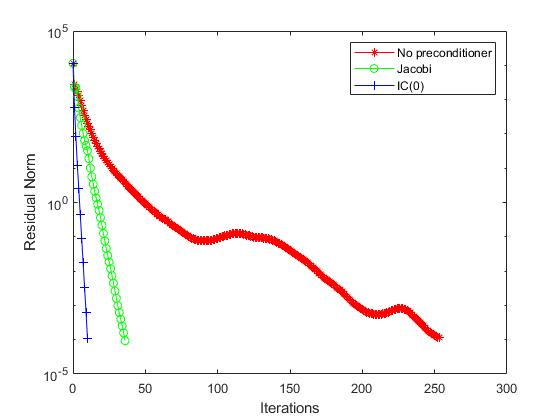
\includegraphics[width=.6\linewidth]{ex4.jpg}
			\caption{semilogy plot ex4}
			\label{fig:ex4}
		\end{figure}
		
		
		\section*{Question 5}
		
		
		\section*{Question 6}
		
		
		\section*{Question 7}
		
		
		\section*{Question 8}
	
	
	
\end{document}



